%% Необхоимый минимум
\documentclass[a4paper,12pt]{article}



%%% Работа с русским языком
\usepackage{cmap}					% поиск в PDF
\usepackage{mathtext} 				% русские буквы в формулах
\usepackage[T2A]{fontenc}			% кодировка
\usepackage[utf8]{inputenc}			% кодировка исходного текста
\usepackage[english,russian]{babel}	% локализация и переносы



%%% Дополнительная работа с математикой
\usepackage{amsfonts,amssymb,amsthm,mathtools} % AMS
\usepackage{amsmath}
\usepackage{icomma} % "Умная" запятая: $0,2$ --- число, $0, 2$ --- перечисление

%% Номера формул
\mathtoolsset{showonlyrefs=true} % Показывать номера только у тех формул, на которые есть \eqref{} в тексте.

%% Шрифты
\usepackage{euscript}	 % Шрифт Евклид
\usepackage{mathrsfs} % Красивый матшрифт

%% Свои команды
\DeclareMathOperator{\sgn}{\mathop{sgn}}

%% Перенос знаков в формулах (по Львовскому)
\newcommand*{\hm}[1]{#1\nobreak\discretionary{}
	{\hbox{$\mathsurround=0pt #1$}}{}}

\usepackage{gensymb}
\usepackage{indentfirst}
\usepackage{lscape}

\usepackage{caption}
\captionsetup{labelsep=period}
\captionsetup{justification=centerlast}
\usepackage{subcaption}
\renewcommand{\thesubfigure}{\asbuk{subfigure}}

\usepackage{microtype}


%%% Параметры страницы: поля, колонтитулы, интерлиньяж
\usepackage{extsizes} % Возможность сделать 14-й шрифт
\usepackage{geometry} % Простой способ задавать поля
\geometry{top=15mm}
\geometry{bottom=15mm}
\geometry{left=15mm}
\geometry{right=15mm}

%\usepackage{fancyhdr} % Колонтитулы
%\pagestyle{fancy}
%\renewcommand{\headrulewidth}{0mm}  % Толщина линейки, отчеркивающей верхний колонтитул
%\lfoot{Нижний левый}
%\rfoot{Нижний правый}
%\rhead{Верхний правый}
%\chead{Верхний в центре}
%\lhead{Верхний левый}
% \cfoot{Нижний в центре} % По умолчанию здесь номер страницы

%\usepackage{setspace} % Интерлиньяж
%\onehalfspacing % Интерлиньяж 1.5
%\doublespacing % Интерлиньяж 2
%\singlespacing % Интерлиньяж 1

%%% Работа с таблицами
\usepackage{array,tabularx,tabulary,booktabs} % Дополнительная работа с таблицами
\usepackage{longtable}  % Длинные таблицы
\usepackage{multirow} % Слияние строк в таблице

%%% Работа с картинками
\usepackage{graphicx}  % Для вставки рисунков
\graphicspath{{images/}{images2/}}  % папки с картинками
\setlength\fboxsep{3pt} % Отступ рамки \fbox{} от рисунка
\setlength\fboxrule{1pt} % Толщина линий рамки \fbox{}
\usepackage{wrapfig} % Обтекание рисунков и таблиц текстом

\usepackage{lastpage} % Узнать, сколько всего страниц в документе.

\usepackage{soul} % Модификаторы начертания
\usepackage{soulutf8} % Модификаторы начертания

%\renewcommand{\familydefault}{\sfdefault} % Начертание шрифта

\usepackage{multicol} % Несколько колонок
\usepackage{listings} %% собственно, это и есть пакет listings
\usepackage{color} %% это для отображения цвета в коде

\lstset{ %
	language=Python,                 % выбор языка для подсветки (здесь это С)
	basicstyle=\small\sffamily, % размер и начертание шрифта для подсветки кода
	numbers=left,               % где поставить нумерацию строк (слева\справа)
	numberstyle=\tiny,           % размер шрифта для номеров строк
	stepnumber=1,                   % размер шага между двумя номерами строк
	numbersep=5pt,                % как далеко отстоят номера строк от подсвечиваемого кода
	backgroundcolor=\color{white}, % цвет фона подсветки - используем \usepackage{color}
	showspaces=false,            % показывать или нет пробелы специальными отступами
	showstringspaces=false,      % показывать или нет пробелы в строках
	showtabs=false,             % показывать или нет табуляцию в строках
	frame=single,              % рисовать рамку вокруг кода
	tabsize=2,                 % размер табуляции по умолчанию равен 2 пробелам
	captionpos=t,              % позиция заголовка вверху [t] или внизу [b] 
	breaklines=true,           % автоматически переносить строки (да\нет)
	breakatwhitespace=false, % переносить строки только если есть пробел
	escapeinside={\%*}{*)}   % если нужно добавить комментарии в коде
}



\newcommand{\signfield}[2]{%
	\rule{#1}{0.1pt}\hspace{-#1}
	\raisebox{-1.1ex}{\parbox[t]{#1}{\centering\scriptsize{#2}}}
}

\begin{document}
\thispagestyle{empty}
\begin{center}
	\large
	{\scshape министерство образования и науки\\российской федерации}
	\vspace{1ex}
	
	{\scshape национальный исследовательский ядерный\\университет <<мифи>>}
	\vspace{4 cm}
	
	\Large
	{\scshape \textbf{О\,Т\,Ч\,Е\,Т}\\о выполнении задания № 2\\<<расчет допустимого энерговыделения в~бочке~с~ЖРО в сухом хранилище>>}
\end{center}

\vspace{4cm}
\begin{flushright}
	\textbf{Выполнил} студент группы С19-103\\
	Мамлеев Антон Алексеевич
	
	\vspace{3 ex}
	\textbf{Руководитель} кандидат технических наук\\
	Куценко Кирилл Владленович
\end{flushright}



\vfill

\begin{center}
	Москва 2023
\end{center}

\newpage

\section{Результаты}

Исследовались зависимости температур бочки, бетонной стенки, а также температуры воздуха в зазоре от энерговыделения в бочке с ЖРО. В результате расчета были получены зависимости, представленные на рис.~\ref{fig:temps}. Также были построены зависимости массового расхода через зазор и коэффициента теплоотдачи от мощности энерговыделения (рис. \ref{fig:G},~\ref{fig:alpha}).

Наиболее важные параметры системы в точках достижения критических температур (вспенивания отходов и охрупчивания бетона) вынесены в таблицу \ref{tab:params}.

\begin{figure}[h]
	\centering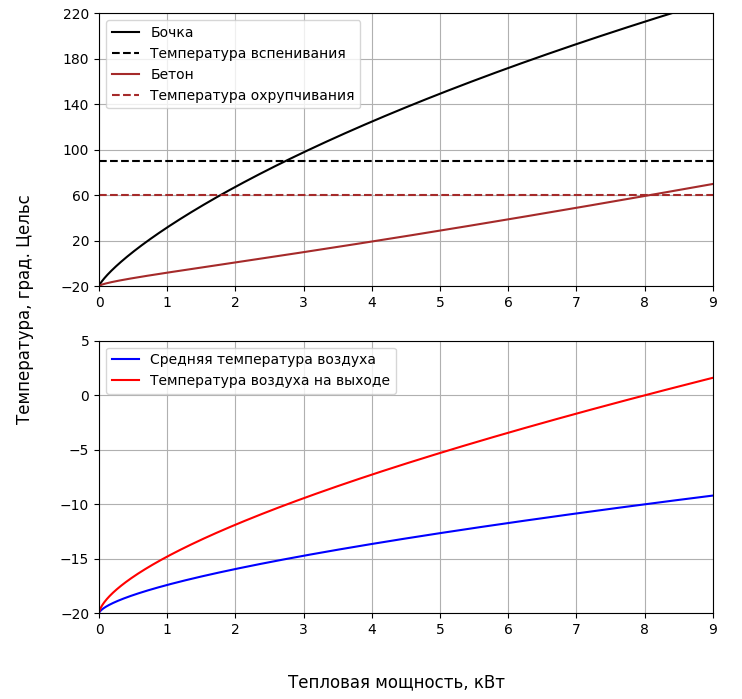
\includegraphics[width=0.9\linewidth]{temps}
	\caption{Графики зависимости температур бочки, бетонной стенки и воздуха от мощности энерговыделения в бочке} \label{fig:temps}
\end{figure}

\begin{figure}[h]
	\centering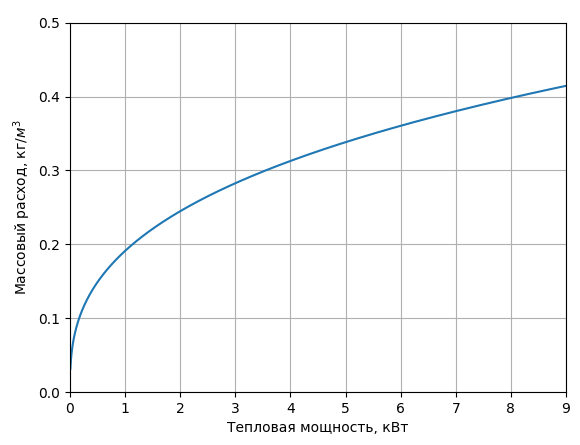
\includegraphics[width=0.6\linewidth]{G}
	\caption{График зависимости массового расхода через зазор от мощности энерговыделения в бочке} \label{fig:G}
\end{figure}

\begin{figure}[h!]
	\centering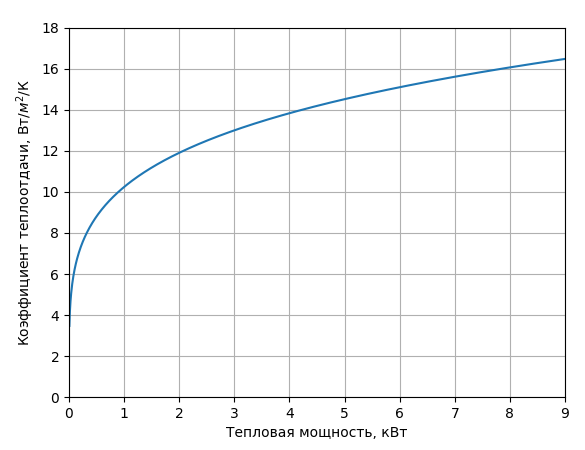
\includegraphics[width=0.6\linewidth]{alpha}
	\caption{График зависимости коэффициента теплоотдачи от мощности энерговыделения в бочке} \label{fig:alpha}
\end{figure}


\begin{table}[h]
	\centering
	\caption{Параметры системы при достижении критических температур} \label{tab:params}
	\begin{tabular}{c|cc}
		\hline
		\begin{tabular}[c]{@{}c@{}}Параметры\\ системы\end{tabular} &
		\begin{tabular}[c]{@{}c@{}}Достижение температуры\\ вспенивания ($t_{боч} = 90~\degree С$)\end{tabular} &
		\begin{tabular}[c]{@{}c@{}}Достижение температуры\\ охрупчивания ($t_{стен} = 60~\degree С$)\end{tabular} \\ \hline
		$Q$, кВт                          & 2.73  & 8.07  \\
		$q_v$, $кВт/м^3$                 & 12.6  & 37.3  \\
		$t_{боч}$, $\degree С$            & 90    & 214   \\
		$t_{стен}$, $\degree С$           & 7.5   & 60.0  \\
		$t_{ср}$, $\degree С$             & -15.0 & -10.0 \\
		$t_{вых}$, $\degree С$            & -10.1 & 0.1   \\
		$\alpha$, $\frac{Вт}{м^2\cdot К}$ & 12.7  & 16.1  \\
		$G$, $кг/с$                       & 0.273 & 0.399 \\ \hline
	\end{tabular}
\end{table}

В отсутствие бетонного ограждения температура вспенивания отходов достигается при меньшем энерговыделении (см. дз. №1): $2.69~кВт$ (с учетом теплоотдачи с торцов) или $2.55~кВт$ (с <<теплоизолированными>> торцами). Таким образом можно сделать вывод, что установка бетонного ограждения позволяет повысить эффективность отвода тепла от бочки с ЖРО.





\end{document}